%*****************************************
\chapter{Working With Data}\label{ch07:data}
%*****************************************

Excel is designed to work with data, and this chapter demonstrates how data is imported and analyzed with tools like pivot tables. The chapter begins with information about validating data input and safeguarding workbooks. 

\section{Safeguarding}

\begin{center}
	\begin{objbox}{Learning Objectives}
		\begin{itemize}
			\setlength{\itemsep}{0pt}
			\setlength{\parskip}{0pt}
			\setlength{\parsep}{0pt}
			
			\item Validate data input to decrease typing errors.
			\item Lock worksheet cells, or entire worksheets, so users do not accidentally change or delete formulas.
			
		\end{itemize}
	\end{objbox}
\end{center}

It is occasionally desirable to safeguard certain cells in a worksheet, or the entire worksheet, to keep a user from accidentally changing something important. For example, if several cells include complex formulas then those should be secured so users will not accidentally delete them. There are two methods generally used to safeguard worksheets: data validation and worksheet protection. 

\subsection{Data Validation}

Excel's data validation rules can be used in a variety of ways.

\begin{itemize}
	\item Restrict the data entered into a cell.
	\item Circle all cells that do not conform to specified validation rules.
	\item Limit the user to a list of possibilities.
\end{itemize}

One of the easiest ways to restrict data is to provide a drop-down list of choices for the user. 

\begin{enumerate}
	\item Open \fmtWorksheet{CH7-Safeguard}.
	\item Save the workbook as \fmtWorksheet{CH7-Protected}.
	\item There is only one worksheet, named \fmtWorksheet{Validation}. Notice there is a list of Zip codes in cells \fmtLoc{K2:K10}. The goal is to permit the user to only select from this list of Zip codes while inputting data in \fmtLoc{Column E} to help reduce data entry errors.
	\item The first step is to name the list of zip codes.
	
	\begin{enumerate}
		\item Select \fmtLoc{K2:K10}.
		\item Click \fmtButton{Formulas $ \Rightarrow $ Defined Names $ \Rightarrow $ Define Name}.
	\end{enumerate}
	
	\begin{figure}[H]
		\centering
		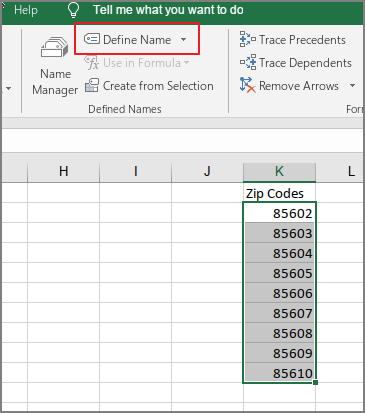
\includegraphics[width=\maxwidth{.75\linewidth}]{gfx/ch07_fig33}
		\caption{Selecting a Range of Cells to Name}
		\label{07:fig33}
	\end{figure}
	
	\begin{enumerate}[resume]		
		\item By default, Excel will suggest the name found in the cell at the top of the range, \fmtLoc{K1} in this case, and that is often acceptable. Notice that Excel replaced the space between ``Zip'' and ``Codes'' with an underscore.
		\item Click \fmtButton{OK}.
		\begin{figure}[H]
			\centering
			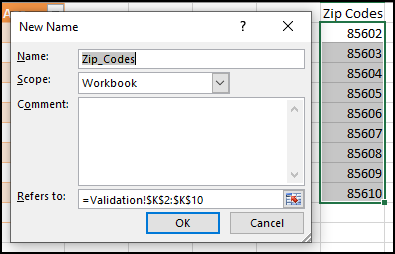
\includegraphics[width=\maxwidth{.85\linewidth}]{gfx/ch07_fig34}
			\caption{Naming a Range of Cells}
			\label{07:fig34}
		\end{figure}
	\end{enumerate}
	
	\item Select \fmtLoc{E2}, which is the first cell that needs data validation. 
	\item Click \fmtButton{Data $ \Rightarrow $ Data Tools $ \Rightarrow $ Data Validation}. (\textit{Note}, click the button, not the down arrow on the right side of the button.)
\end{enumerate}

\begin{figure}[H]
	\centering
	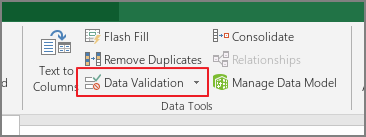
\includegraphics[width=\maxwidth{.75\linewidth}]{gfx/ch07_fig35}
	\caption{The Data Validation Button}
	\label{07:fig35}
\end{figure}

\begin{enumerate}[resume]	
	\item Select \fmtButton{List} in the \textit{Allow} field.
\end{enumerate}

\begin{figure}[H]
	\centering
	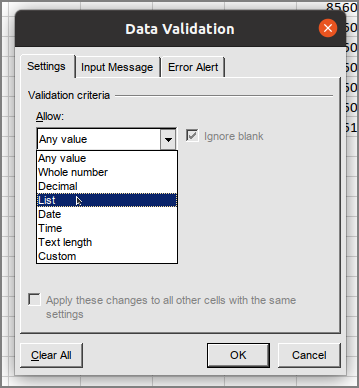
\includegraphics[width=\maxwidth{.75\linewidth}]{gfx/ch07_fig36}
	\caption{Selecting A Validation List}
	\label{07:fig36}
\end{figure}

\begin{enumerate}[resume]	
	\item Check \fmtButton{Ignore blank}. If this is left unchecked then it would force the user to enter a zip code, but when this is checked the user can leave the zip code field blank.
	\item Check \fmtButton{In-cell dropdown}. This creates a drop-down list so the user can select a zip code from a list rather than enter it manually.
	\item Enter \fmtTyping{=Zip\_Codes} for the \textit{Source} (notice the underscore between the word ``Zip'' and ``Codes''). This tells Excel that the acceptable list of zip codes for cell \fmtLoc{E2} is found in the \textit{Zip Codes} list.
	\item Click \fmtButton{OK}.
\end{enumerate}

\begin{figure}[H]
	\centering
	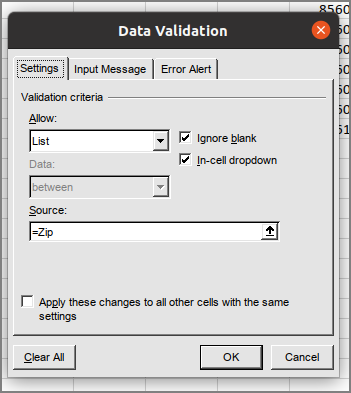
\includegraphics[width=\maxwidth{.75\linewidth}]{gfx/ch07_fig37}
	\caption{Setting the Data Validation List}
	\label{07:fig37}
\end{figure}

After following the above steps, a drop-down selection box will appear whenever the user clicks into cell \fmtLoc{E2}, as illustrated in Figure \ref{07:fig38}. 

\begin{figure}[H]
	\centering
	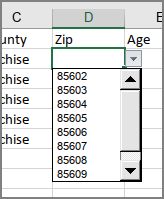
\includegraphics[width=\maxwidth{.95\linewidth}]{gfx/ch07_fig38}
	\caption{Valid Selections}
	\label{07:fig38}
\end{figure}

\begin{enumerate}[resume]
	\item Copy \fmtLoc{E2} to \fmtLoc{E3:E11} so all of those cells will also get the drop-down \textit{Zip Codes} validation list.
	\item Select any of the \textit{Zip Codes} to fill \fmtLoc{E2:E11}.
\end{enumerate}

\begin{center}
	\begin{infobox}{Note}
		\textbf{Validation List Location}
		\\
		\\
		For this exercise the list of valid zip codes was contained on the same worksheet as the cells to be validated. However, the validation list is normally found on a different worksheet so it can be protected and, optionally, hidden from the user.
	\end{infobox}
\end{center}

A second validation method is used when the user can enter data that cannot be selected from a list. For example, if users are required to enter their age then a drop-down list containing every possible age is not reasonable. In this case, Excel can be set up to ensure that the data entered is within certain specific bounds. For example, an ``age'' entry could be between $ 20 $ and $ 65 $ for working adults (or maybe some other range). Data validation can use a full set of Boolean comparisons (between, equal to, greater than, etc.). As part of the process, various messages can be displayed when the cell is selected to help guide the user. Finally, the action taken when invalid data is entered (\textit{Stop}, \textit{Warning}, or \textit{Information}) can be specified.

\begin{enumerate}
	\item Notice that the \fmtWorksheet{Validation} worksheet includes an entry for \textit{Age}. The expectation is that users will enter their age but it is important to restrict this data to numbers between $ 20 $ and $ 65 $ so they do not accidentally enter a number out of the range or even text.
	\item Select \fmtLoc{F2}, which is the first cell that needs data validation. 
	\item Click \fmtButton{Data $ \Rightarrow $ Data Tools $ \Rightarrow $ Data Validation}. (\textit{Note}, click the button, not the down arrow on the right side of the button.)
	\item Select \fmtButton{Whole number} in the \textit{Allow} field.
	\item Select \fmtButton{Between} in the \textit{Data} field.
	\item Enter \fmtTyping{20} in the \textit{Minimum} field.
	\item Enter \fmtTyping{65} in the \textit{Maximum} field.
\end{enumerate}

\begin{figure}[H]
	\centering
	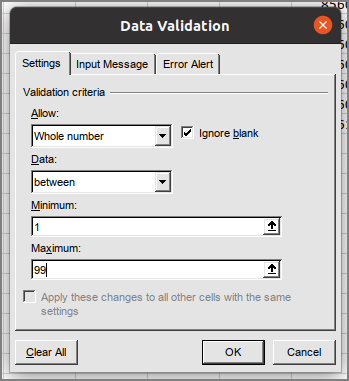
\includegraphics[width=\maxwidth{.75\linewidth}]{gfx/ch07_fig39}
	\caption{Settings for Validating Numeric Data}
	\label{07:fig39}
\end{figure}

\begin{enumerate}[resume]	
	\item Click the \textit{Input Message} tab and enter \fmtTyping{Age} for the \textit{Title} and \fmtTyping{Input an age between $ 20 $ and $ 65 $.} for the \textit{Input Message}.
	\item Click the \textit{Error Alert} tab and select the \fmtButton{Stop} style then enter \fmtTyping{Age} for the \textit{Title} and \fmtTyping{Input an age between $ 20 $ and $ 65 $.} for the \textit{Input Message}.
	\item Click \fmtButton{OK}.
	\item Copy \fmtLoc{F2} to \fmtLoc{F3:F11}.
	\item Click in \fmtLoc{F2} to activate that cell. Notice that the help message pops up. Enter some number in \fmtLoc{F2}. If that number is between $ 20 $ and $ 65 $ then the entry works without error, but if anything else is entered an error message pops up and forces a correct number to be entered.
	\item Enter $ 19 $ in \fmtLoc{F2} to force an error.
	\item Click \fmtButton{Cancel} on the \textit{Age} error message.
	\item Delete the data in \fmtLoc{F2}.
\end{enumerate}

\begin{figure}[H]
	\centering
	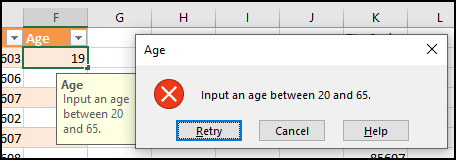
\includegraphics[width=\maxwidth{.75\linewidth}]{gfx/ch07_fig40}
	\caption{Stopping on Data Entry Error}
	\label{07:fig40}
\end{figure}

\begin{enumerate}[resume]	
	\item Click \fmtLoc{F2} to activate that cell.
	\item Click \fmtButton{Data $ \Rightarrow $ Data Tools $ \Rightarrow $ Data Validation}. (\textit{Note}, click the button, not the down arrow on the right side of the button.)
	\item Click the \textit{Error Alert} tab on the \textit{Data Validation} dialog box. 
	\item This cell was initially set to \textit{Stop} on an error. Perhaps, though, it would be acceptable for the user to finish the data entry even if it contained an error. Change the Style drop-down to \fmtButton{Warning}.
	\item Click \fmtButton{OK}.
	\item Copy \fmtLoc{F2} to \fmtLoc{F3:F11}.
	\item Click in \fmtLoc{F2} to activate that cell. Notice that the help message pops up. Enter some number in \fmtLoc{F2}. If that number is between $ 20 $ and $ 65 $ then the entry works without error, but if anything else is entered a warning message pops up and permits the user to continue with the bad number or retry.
\end{enumerate}

\begin{figure}[H]
	\centering
	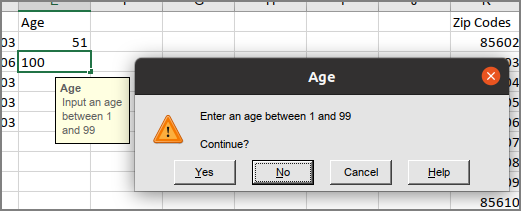
\includegraphics[width=\maxwidth{.95\linewidth}]{gfx/ch07_fig41}
	\caption{Warning on Data Entry Error}
	\label{07:fig41}
\end{figure}

\begin{enumerate}[resume]	
	\item Enter these numbers into cells \fmtLoc{F2:F11}: \fmtTyping{$ 19 $, $ 50 $, $ 67 $, $ 40 $, $ 53 $, $ 35 $, $ 60 $, $ 23 $, $ 65 $, $ 21 $}. A warning should pop up for \fmtLoc{F2} and \fmtLoc{F4} since those entries are out of the acceptable range, but click \fmtButton{Yes} on the warning popup box so the data is entered.
	\item Click \fmtButton{Data $ \Rightarrow $ Data Tools $ \Rightarrow $ $ \Rightarrow $ Data Validation Down Arrow $ \Rightarrow $ Circle Invalid Data}.
\end{enumerate}

\begin{figure}[H]
	\centering
	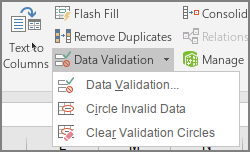
\includegraphics[width=\maxwidth{.50\linewidth}]{gfx/ch07_fig42}
	\caption{Data Validation Options}
	\label{07:fig42}
\end{figure}

\begin{enumerate}[resume]	
	\item Notice that the cells containing bad data are now circled so they can be corrected.
\end{enumerate}

\begin{figure}[H]
	\centering
	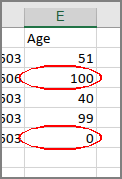
\includegraphics[width=\maxwidth{.95\linewidth}]{gfx/ch07_fig43}
	\caption{Circled Data Errors}
	\label{07:fig43}
\end{figure}

\begin{enumerate}[resume]	
	\item Click \fmtButton{Data $ \Rightarrow $ Data Tools $ \Rightarrow $ Data Validation Down Arrow $ \Rightarrow $ Clear Validation Circles} to clear the validation circles.
\end{enumerate}

\begin{center}
	\begin{infobox}{Note}
		\textbf{Data Validation}
		\\
		\\
		Data validation will not automatically update the error circles as new data is entered. Therefore, after data is entered into a worksheet the \textit{Circle Invalid Data} button must be clicked to check that data.
	\end{infobox}
\end{center}

\subsection{Worksheet Protection}

After entering the data validation rules, it may be desirable to lock the \fmtWorksheet{Validation} worksheet so users cannot accidentally delete the formulas or change the \textit{Zip Codes} validation list. Before adding protection to a worksheet, cells that need to remain open for editing must be unlocked. That way, after the entire sheet is locked those selected cells can still be edited. Follow these steps to unlock cells that should remain editable. 

\begin{enumerate}
	\item Select \fmtLoc{A2:F11}. These are the only cells that users should be able to modify.
	\item Click \fmtButton{Home $ \Rightarrow $ Cells $ \Rightarrow $ Format $ \Rightarrow $ Lock Cell}.
	\item Click cell \fmtLoc{A2}.
	\item Click \fmtButton{Home $ \Rightarrow $ Cells $ \Rightarrow $ Format $ \Rightarrow $ Protect Sheet}.
	\item On the \textit{Protect Sheet} dialog box, check \fmtButton{Protect worksheet and contents of locked cells}.
	\item Uncheck all options except \fmtButton{Select Unlocked Cells}.
	\item Click \fmtButton{OK}.
	\item Notice that now the mouse cannot click in any cell except \fmtLoc{A2:F11}
	\item Save and close the \fmtWorksheet{CH7-Protected} workbook.
\end{enumerate}

\begin{center}
	\begin{infobox}{Important!}
		\textbf{About Passwords}
		\\
		\\
		Worksheets can be password protected, but there is no way to recover the worksheet if the password is forgotten. Therefore, it is essential to use a password that is easy to remember but difficult to guess.
	\end{infobox}
\end{center}

\begin{center}
	\begin{infobox}{Important!}
		\textbf{Security}
		\\
		\\
		While it is easy to lock worksheets to keep users from accidentally changing a formula, this should not be considered any sort of security. Users can easily unlock the worksheet and make whatever changes they want. This is just a way to stop users from accidentally making changes.
	\end{infobox}
\end{center}

\begin{center}
	\begin{tkwbox}{Key Take-Aways}
		\textbf{Safeguarding}
		\\
		\begin{itemize}
			\setlength{\itemsep}{0pt}
			\setlength{\parskip}{0pt}
			\setlength{\parsep}{0pt}
			
			\item Data entry can be validated to decrease the chance of bad data being entered due to simple typing errors.
			\item Worksheets can be protected so users cannot accidentally change formulas or data.
			
		\end{itemize}
	\end{tkwbox}
\end{center}

\section{Importing Data}

\begin{center}
	\begin{objbox}{Learning Objectives}
		\begin{itemize}
			\setlength{\itemsep}{0pt}
			\setlength{\parskip}{0pt}
			\setlength{\parsep}{0pt}
			
			\item Import data from the web and local files.

		\end{itemize}
	\end{objbox}
\end{center}

To use Excel's powerful tools for analysis, data must first be imported into a spreadsheet. Data can be imported from many sources but two common ones are from the web and from a datafile located on the local computer. Data is very often posted on the web for researchers to use in their projects. The United States federal government, for example, has more than $ 200,000 $ datasets freely available in fields like taxes, crime, trade, education, and dozens of other topics\footnote{See \url{https://www.data.gov/}}. Sometimes, that data can be imported directly into Excel but more often it must be downloaded to a local computer and then imported into Excel from that file. This section demonstrates both of those procedures.

\subsection{Import From the Web}

Data contained in a table on a website can be imported directly into an Excel workbook. Follow these steps to import data from a website.

\begin{enumerate}
	\item Open a new blank workbook.
\end{enumerate}

\begin{center}
	\begin{infobox}{Note}
		\textbf{Downloading From the Web}
		\\
		\\
		\fmtOldExcel{Excel 2016} includes a feature to get data from the web at \textit{Data $ \Rightarrow $ Get External Data $ \Rightarrow $ From Web}, as shown in Figure \ref{07:fig01}. Unfortunately, that feature relies on the computer's browser and Excel's download function is blocked by modern browsers. Therefore, the process described in this section is the only way to reliably download data from the web into Excel.
	\end{infobox}
\end{center}

\begin{figure}[H]
	\centering
	\includegraphics[width=\maxwidth{.75\linewidth}]{gfx/ch07_fig01}
	\caption{Import From Web Menu}
	\label{07:fig01}
\end{figure}

For this exercise, the ``Juggling World Records'' page on Wikipedia will be used since it includes several different tables.

\begin{enumerate}[resume]
	\item \fmtOldExcel{Excel 2016} Click \fmtButton{Data $ \Rightarrow $ Get \& Transform $ \Rightarrow $ New Query $ \Rightarrow $ From Other Sources $ \Rightarrow $ From Web}
	\item \fmtNewExcel{Excel 365} Click \fmtButton{Data $ \Rightarrow $ Get \& Transform Data $ \Rightarrow $ Get Data $ \Rightarrow $ From Other Sources $ \Rightarrow $ From Web}
	\item Select the \fmtButton{Basic} option and enter \fmtTyping{https://bit.ly/AdExcelC} in the \textit{From Web} popup, as shown in Figure \ref{07:fig02a}.
\end{enumerate}
	
\begin{figure}[H]
	\centering
	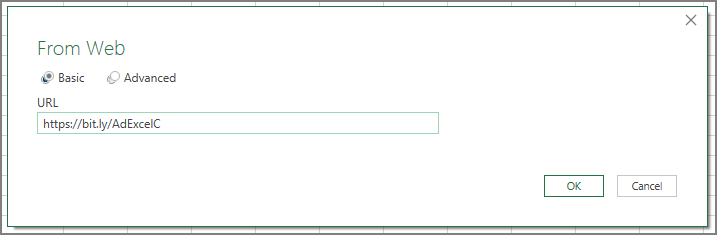
\includegraphics[width=\maxwidth{.95\linewidth}]{gfx/ch07_fig02a}
	\caption{From Web URL Window}
	\label{07:fig02a}
\end{figure}
	
\begin{enumerate}[resume]
	\item Press \fmtButton{OK}
	\item It may take a few seconds for Excel to make a connection.
	\item Excel permits several options to be set before accessing the Web content, but the defaults are acceptable. Click \fmtButton{Connect}.
\end{enumerate}

\begin{figure}[H]
	\centering
	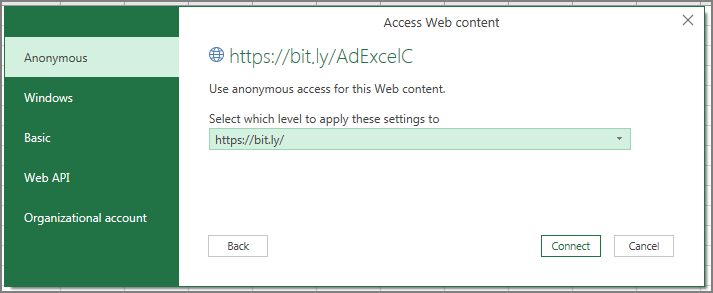
\includegraphics[width=\maxwidth{.95\linewidth}]{gfx/ch07_fig02g}
	\caption{Access Web Content Options}
	\label{07:fig02g}
\end{figure}
	
\begin{enumerate}[resume]
	\item A box will popup with a list of all tables on the page. In Figure \ref{07:fig02b}, the first table has been selected and a preview of that table can be seen.
\end{enumerate}

\begin{figure}[H]
	\centering
	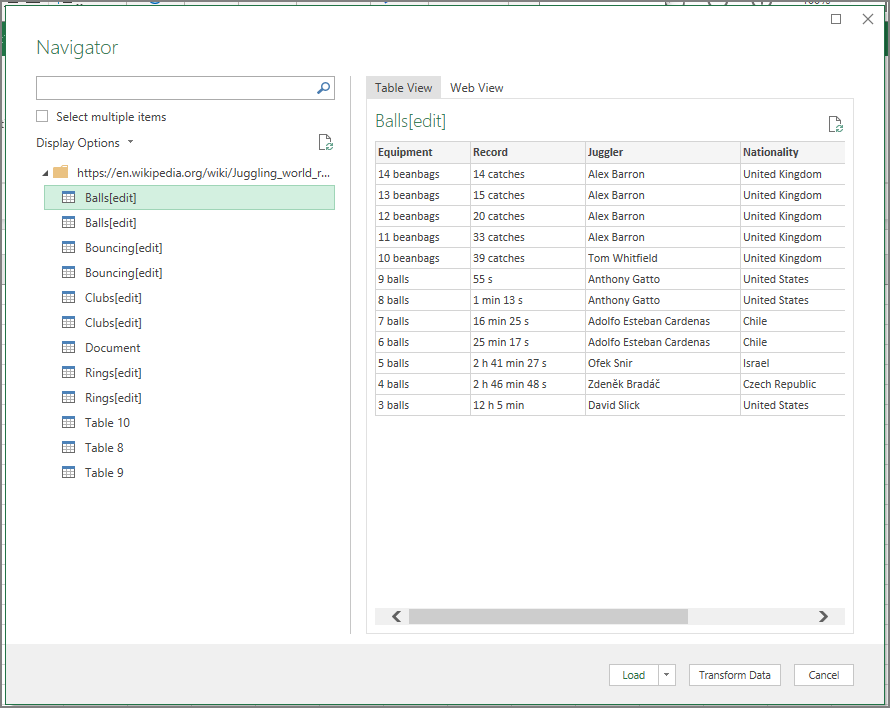
\includegraphics[width=\maxwidth{.95\linewidth}]{gfx/ch07_fig02b}
	\caption{Listing of Webpage Tables}
	\label{07:fig02b}
\end{figure}

\begin{enumerate}[resume]
	\item Select the first table and click \fmtButton{Load}
	\item After Excel retrieves the data, it is imported into a table on a new worksheet, as shown in Figure \ref{07:fig02c}.
\end{enumerate}

\begin{figure}[H]
	\centering
	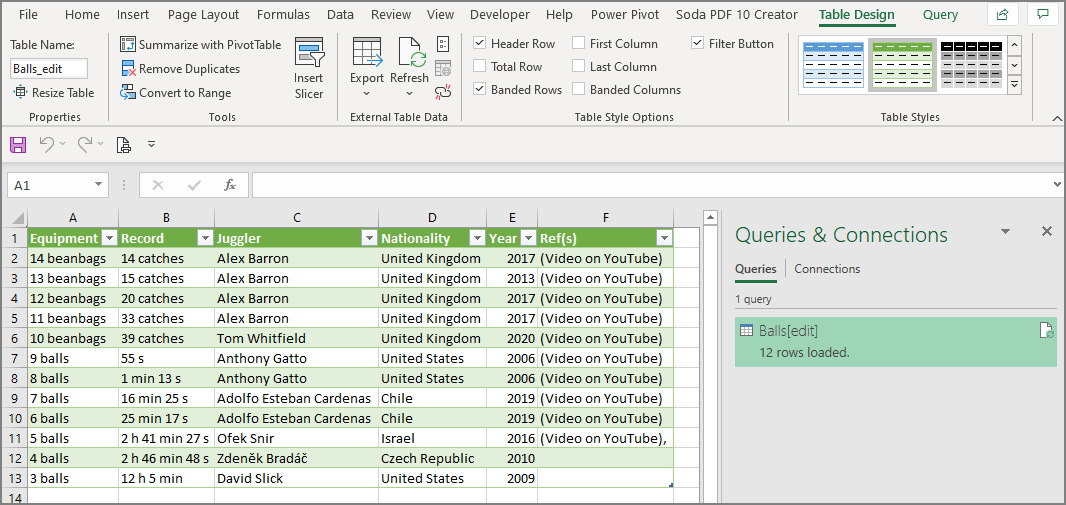
\includegraphics[width=\maxwidth{.95\linewidth}]{gfx/ch07_fig02c}
	\caption{Imported Data Table}
	\label{07:fig02c}
\end{figure}

The imported data contains records for number of balls juggled as found on a Wikipedia page. Excel displays a \textit{Queries \& Connections} box on the right side of the screen. That box lists the Web queries that were used to import data tables. Since there has only been one query then only one item appears in this box, but if more queries are run they will also be listed here. 

\begin{enumerate}[resume]
	\item Close the \textit{Queries \& Connections} box by clicking the \fmtButton{X} in the top right corner of the box.
	\item Delete the \fmtWorksheet{Sheet1} worksheet.
	\item Rename the \fmtWorksheet{Sheet2} worksheet to \fmtWorksheet{Juggling}.
\end{enumerate}

The webpage data is imported into Excel as a table, so tools like filtering, sorting, and slicing the data are readily available. As with any Excel table, this data table can be recolored and formatted as desired\footnote{See Chapter \ref{ch05:tables}, \nameref{ch05:tables}, page \pageref{ch05:tables} for more information about tables.}.

\subsection{Transforming Data}

Normally, raw data includes unnecessary rows and columns that will need to be ``cleaned up'' a bit before it can be imported. This is a process that is called \textit{Transforming} and Excel makes that process easy to complete. 

\begin{enumerate}
	\item \fmtOldExcel{Excel 2016} Click \fmtButton{Data $ \Rightarrow $ Get \& Transform $ \Rightarrow $ New Query $ \Rightarrow $ From Other Sources $ \Rightarrow $ From Web}
	\item \fmtNewExcel{Excel 365} Click \fmtButton{Data $ \Rightarrow $ Get \& Transform Data $ \Rightarrow $ Get Data $ \Rightarrow $ From Other Sources $ \Rightarrow $ From Web}
	\item Enter \fmtTyping{https://bit.ly/AdExcelB} in the \textit{From Web} popup, as shown in Figure \ref{07:fig02a} and click \fmtButton{OK}.
	\item For this exercise, an online table with FBI crime statistics from $ 2017 $ is being used as a source. Select Table $ 0 $, as shown in Figure \ref{07:fig02d}.
	\item Notice in the preview that this table includes crime statistics for the years $ 2016 $ and $ 2017 $. It also includes various non-state regions, like ``Northeast.'' For this exercise, only the state-level data for $ 2017 $ is needed and it is much easier to filter that before the data is imported than to remove it later.
	\item \fmtOldExcel{Excel 2016} Click \fmtButton{Edit} under the preview area.
	\item \fmtNewExcel{Excel 365} Click \fmtButton{Transform Data} under the preview area.
\end{enumerate}

\begin{figure}[H]
	\centering
	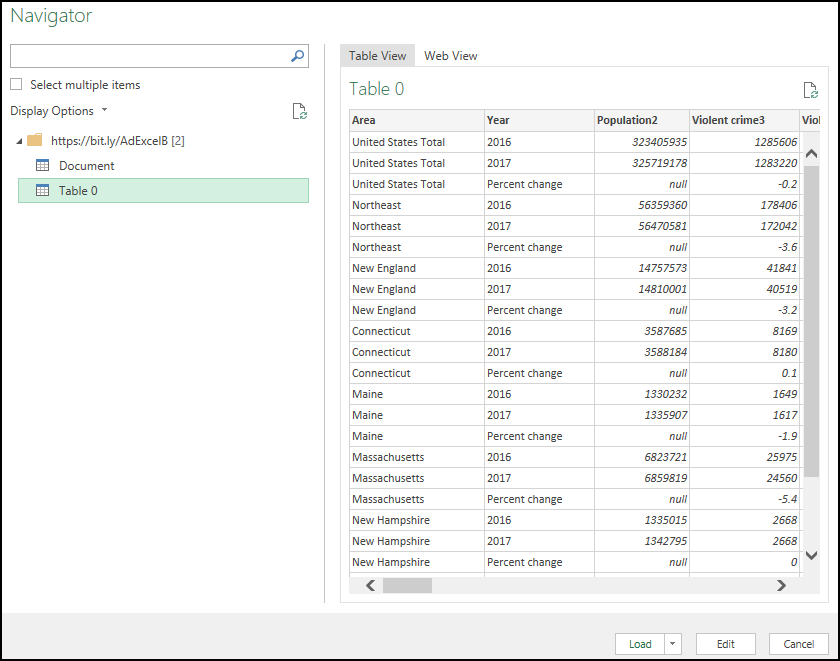
\includegraphics[width=\maxwidth{.95\linewidth}]{gfx/ch07_fig02d}
	\caption{Selecting Table 0}
	\label{07:fig02d}
\end{figure}

\begin{enumerate}[resume]
	\item The \textit{Microsoft Power Query Editor} window pops up where the data can be filtered and edited in many ways before it is imported. For this exercise, only two simple filters will be applied.
\end{enumerate}

\begin{figure}[H]
	\centering
	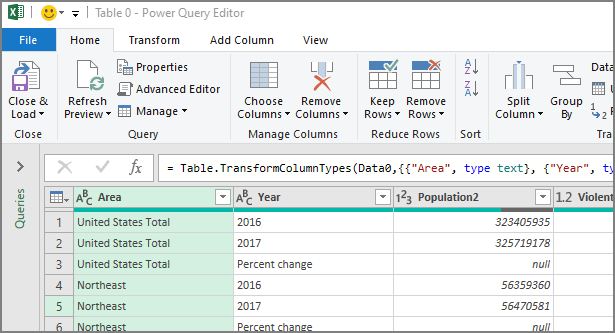
\includegraphics[width=\maxwidth{.95\linewidth}]{gfx/ch07_fig02e}
	\caption{Power Query Editor}
	\label{07:fig02e}
\end{figure}

\begin{enumerate}[resume]
	\item Click the down arrow beside the \textit{Year} column heading and select only $ 2017 $ data and then click \fmtButton{OK}.
\end{enumerate}

\begin{figure}[H]
	\centering
	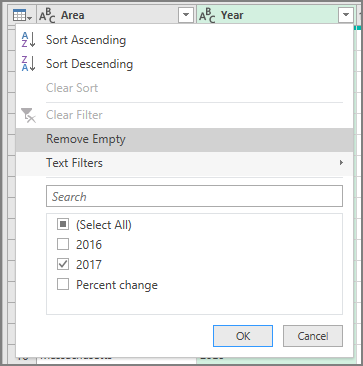
\includegraphics[width=\maxwidth{.75\linewidth}]{gfx/ch07_fig02f}
	\caption{Filtering on 2017 Records}
	\label{07:fig02f}
\end{figure}

\begin{enumerate}[resume]
	\item In the same way, click the down arrow beside the \textit{Area} column heading and uncheck all rows that are not state names, like ``East North Central,'' and then click \fmtButton{OK}. (Note: leave \textit{District of Columbia} and \textit{Puerto Rico} in the list.)
	\item Click \fmtButton{Home $ \Rightarrow $ Close $ \Rightarrow $ Close \& Load}
	\item Excel loads the data in a table on a new sheet. Rename the worksheet to \fmtWorksheet{Crime}.
	\item Save the workbook as \fmtWorksheet{CH7-WebData.xlsx}.
	\item Close \fmtWorksheet{CH7-WebData.xlsx}.
\end{enumerate}

\subsection{Import From Data File}\label{07:ImportFromDataFile}

It is common for web data to be downloaded via a data file. Those data files are, typically, in a \textit{.CSV} format (that stands for ``Comma Separated Values''). This is a simple text file and can be opened with a program no more complicated than \textit{Notepad}; but \textit{.CSV} files are typically opened with Excel or some other data analysis tool. Figure \ref{07:fig04} shows the first few lines of the sales data file used in this lesson opened in \textit{Notepad}.

\begin{figure}[H]
	\centering
	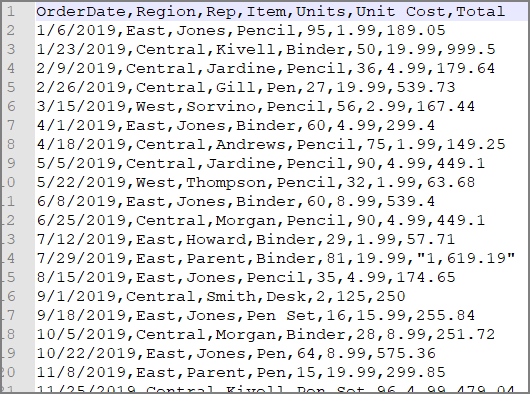
\includegraphics[width=\maxwidth{.95\linewidth}]{gfx/ch07_fig04}
	\caption{CSV File}
	\label{07:fig04}
\end{figure}

Complete the following steps to load a \textit{.CSV} file into Excel.

\begin{enumerate}
	\item Open a new blank workbook.
	\item \fmtOldExcel{Excel 2016} Click \fmtButton{Data $ \Rightarrow $ Get \& Transform $ \Rightarrow $ New Query $ \Rightarrow $ From File $ \Rightarrow $ From CSV}.
	\item \fmtNewExcel{Excel 365} Click \fmtButton{Data $ \Rightarrow $ Get \& Transform Data $ \Rightarrow $ Get Data $ \Rightarrow $ From File $ \Rightarrow $ From Text/CSV}
	Figure \ref{07:fig05a} illustrates this button.
\end{enumerate}

\begin{figure}[H]
	\centering
	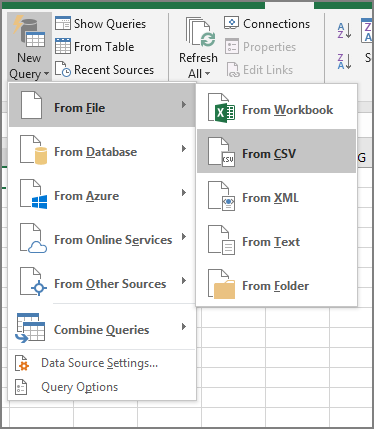
\includegraphics[width=\maxwidth{.65\linewidth}]{gfx/ch07_fig05a}
	\caption{Import CSV File}
	\label{07:fig05a}
\end{figure}

\begin{enumerate}[resume]
	\item Navigate to \fmtWorksheet{CH7-Data.csv}.
	\item Click the file name and then \fmtButton{Import}. Figure \ref{07:fig06} shows the \textit{Import Data} dialog box.
\end{enumerate}

\begin{figure}[H]
	\centering
	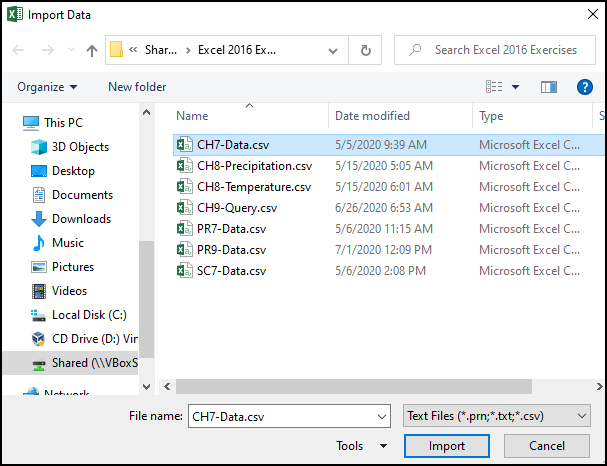
\includegraphics[width=\maxwidth{.95\linewidth}]{gfx/ch07_fig06}
	\caption{Selecting the CSV file}
	\label{07:fig06}
\end{figure}

\begin{enumerate}[resume]
	\item Excel will begin to import the .CSV data. Excel makes its ``best guess'' about the type of data in the file, as illustrated in Figure \ref{07:fig07a}.
\end{enumerate}

\begin{figure}[H]
	\centering
	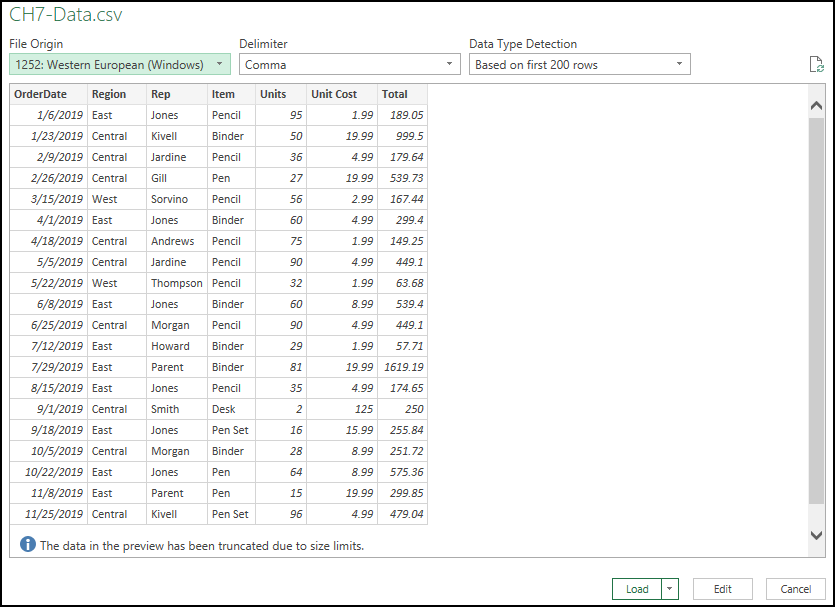
\includegraphics[width=\maxwidth{.95\linewidth}]{gfx/ch07_fig07a}
	\caption{CSV Import Wizard}
	\label{07:fig07a}
\end{figure}

\begin{enumerate}[resume]
	\item The sample text contained in the box illustrated in Figure \ref{07:fig07a} looks correct, so Excel has correctly determined that the CSV file contains ``1252 Western European (Windows)'' text that uses a comma delimiter. Click \fmtButton{Load}.
	\item Excel loads the .CSV data into a new worksheet.
	\item Close the \textit{Queries \& Connections} panel by clicking the \fmtButton{X} in the top right corner of the box.
\end{enumerate}

Figure \ref{07:fig10} shows the first few lines of the worksheet which has the imported data in a table that can be manipulated like any other table.

\begin{figure}[H]
	\centering
	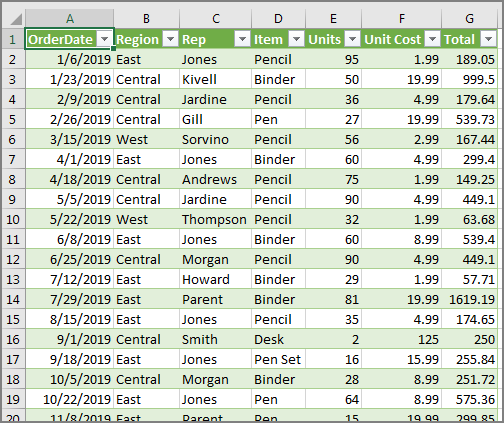
\includegraphics[width=\maxwidth{.95\linewidth}]{gfx/ch07_fig10}
	\caption{The Worksheet With Imported Data}
	\label{07:fig10}
\end{figure}

\begin{enumerate}[resume]
	\item Rename \fmtWorksheet{Sheet2} to \fmtWorksheet{Sales Data}.
	\item Delete \fmtWorksheet{Sheet1}.
	\item Save the workbook as \fmtWorksheet{CH7-Sales Summary}.
\end{enumerate}

\begin{center}
	\begin{tkwbox}{Key Take-Aways}
		\textbf{Importing Data}
		\\
		\begin{itemize}
			\setlength{\itemsep}{0pt}
			\setlength{\parskip}{0pt}
			\setlength{\parsep}{0pt}
			
			\item Data can be imported from tables found on websites using \textit{Data $ \Rightarrow $ Get External Data $ \Rightarrow $ From Web}. 
			\item Data can be imported from CSV files downloaded from websites using \textit{Data $ \Rightarrow $ Get \& Transform $ \Rightarrow $ New Query $ \Rightarrow $ From File $ \Rightarrow $ From CSV}.
			
		\end{itemize}
	\end{tkwbox}
\end{center}

\section{Pivot Tables}

\begin{center}
	\begin{objbox}{Learning Objectives}
		\begin{itemize}
			\setlength{\itemsep}{0pt}
			\setlength{\parskip}{0pt}
			\setlength{\parsep}{0pt}

			\item Create a pivot table.
			\item Manipulate a pivot table to change the information displayed.
			
		\end{itemize}
	\end{objbox}
\end{center}

Pivot tables dynamically summarize data and are a favorite tool for analysts since they are highly customizable and very powerful. These tools are called pivot tables because the data displayed can be easily pivoted from rows to columns and back. Pivot tables are sometimes called contingency tables or crosstabs and are frequently seen in reports where tabular data is presented. A common example of a pivot table is found in newspapers and magazines during elections where the editor creates a table showing the number of voters by party, gender, race, or other factors. For this exercise, sales data from a small supplier will be analyzed.

\begin{enumerate}
	\item Open the \fmtWorksheet{Sales Summary} workbook that was created in section \ref{07:ImportFromDataFile} if it is not already opened.
	\item Click in cell \fmtLoc{A1} in the \fmtWorksheet{Sales Data} worksheet.
	\item Click \fmtButton{Insert $ \Rightarrow $ Tables $ \Rightarrow $ PivotTable}. In Figure \ref{07:fig11}, the \fmtButton{PivotTable} button can be found at the left end of the ribbon.
\end{enumerate}

\begin{figure}[H]
	\centering
	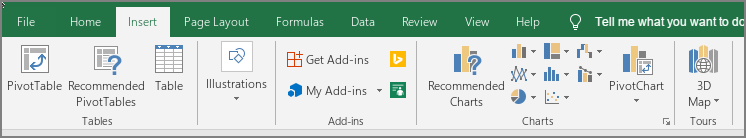
\includegraphics[width=\maxwidth{.75\linewidth}]{gfx/ch07_fig11}
	\caption{PivotTable Button On The Ribbon}
	\label{07:fig11}
\end{figure}

\begin{enumerate}[resume]
	\item In the \textit{Create PivotTable} popup, as seen in Figure \ref{07:fig12}, ensure that Excel automatically selected either the name of the data table, \textit{CH7\_Data}, or the range \$A\$1:\$G\$44, which is all the data on the worksheet. Also, ensure \fmtButton{New Worksheet} is selected as the location of the new pivot table. 
	\item Click \fmtButton{OK}.
\end{enumerate}

\begin{figure}[H]
	\centering
	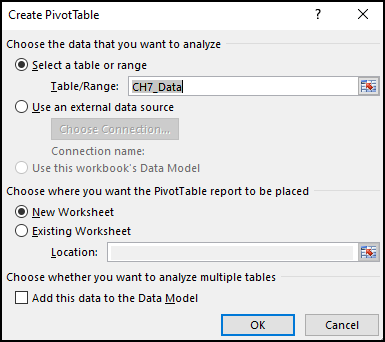
\includegraphics[width=\maxwidth{.75\linewidth}]{gfx/ch07_fig12}
	\caption{Create PivotTable Wizard}
	\label{07:fig12}
\end{figure}


\begin{enumerate}[resume]
	\item A pivot table is created on a new worksheet. Rename that sheet \fmtWorksheet{Sales Pivot}.
	\item Move the \fmtWorksheet{Sales Pivot} worksheet to the right of \fmtWorksheet{Sales Data} if it is not already placed there.
	\item A blank pivot table has six areas of interest for this lesson, as shown in Figure \ref{07:fig13}.

	\begin{itemize}
		\item \textbf{A}. The \textbf{Pivot Table} will appear in the large area on the left (it is blank in the illustration).
		\item \textbf{B}. The \textbf{Field List} contains the names of all the fields available in the data set. These are the column headers in the data table.
		\item \textbf{C}. \textbf{Filters} is where complex filters can be created to restrict the data displayed on the pivot table.
		\item \textbf{D}. \textbf{Column Labels} define the columns on the pivot table.
		\item \textbf{E}. \textbf{Row Labels} define the rows on the pivot table.
		\item \textbf{F}. \textbf{Values} define the numeric data calculated and displayed in the pivot table.
	\end{itemize}
\end{enumerate}

\begin{figure}[H]
	\centering
	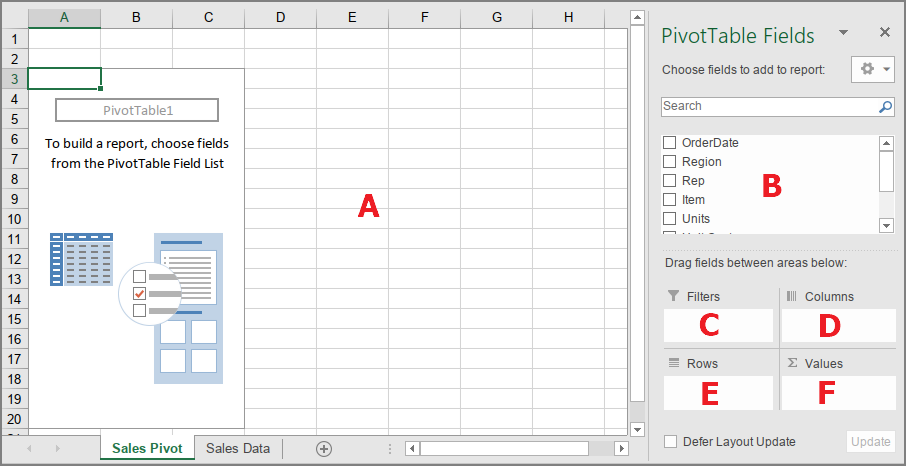
\includegraphics[width=\maxwidth{.95\linewidth}]{gfx/ch07_fig13}
	\caption{Pivot Table Areas}
	\label{07:fig13}
\end{figure}

\begin{enumerate}[resume]
	\item Drag and drop \textit{Region} in the \textit{Field List} to the \textit{Rows} area. 
	\item Drag and drop \textit{Item} in the \textit{Field List} to the \textit{Rows} area under \textit{Region}.
	\item Drag and drop \textit{Units} in the \textit{Field List} to the \textit{Values} area. Excel automatically displays the number of units sold for each item,  the total sold by region, and a Grand Total. With just a few clicks of the mouse, Excel has created a useful decision-making chart for managers. Figure \ref{07:fig14} illustrates the pivot table at this point.
\end{enumerate}

\begin{figure}[H]
	\centering
	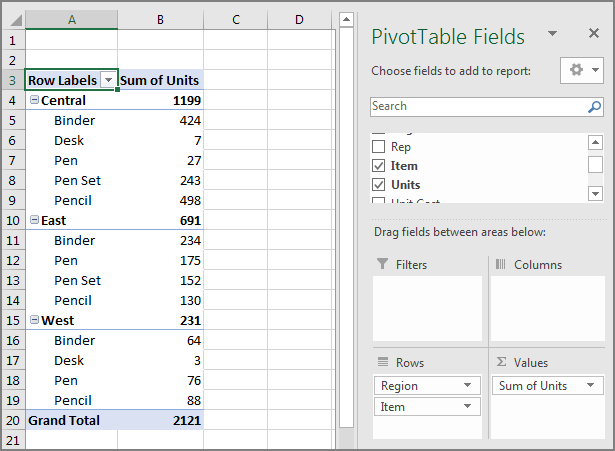
\includegraphics[width=\maxwidth{.95\linewidth}]{gfx/ch07_fig14}
	\caption{Sales Units}
	\label{07:fig14}
\end{figure}
	
\begin{enumerate}[resume]
	\item Click and drag \textit{Item} from the \textit{Row Labels} area to the \textit{Column Labels} area. (Note, this can also be done by clicking the down-arrow for \textit{Item} and selecting \fmtButton{Move to Column Labels}.) The same data is still being displayed, but it has been rearranged to make it easier to compare regions. Also notice that Excel automatically created two Grand Totals, one for the rows and one for the columns. Figure \ref{07:fig15} illustrates the pivot table at this point.
\end{enumerate}	

\begin{figure}[H]
	\centering
	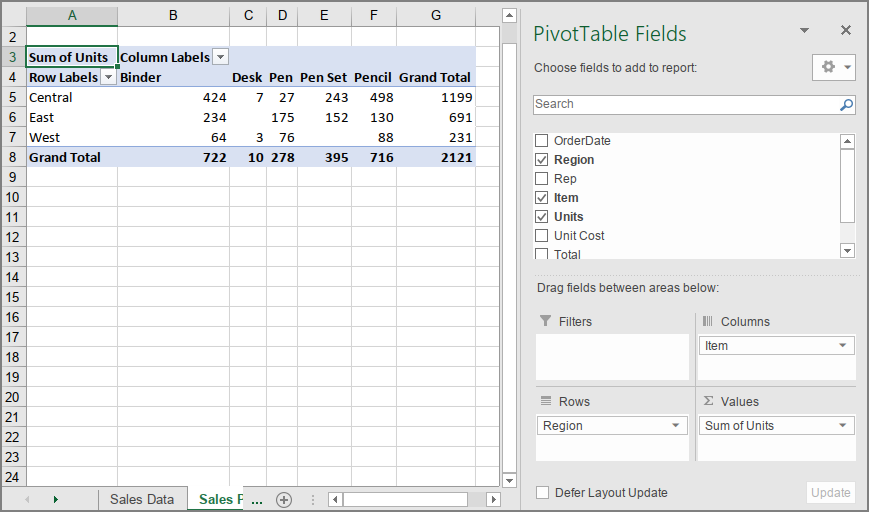
\includegraphics[width=\maxwidth{.95\linewidth}]{gfx/ch07_fig15}
	\caption{Sales Units With Columns}
	\label{07:fig15}
\end{figure}

\begin{enumerate}[resume]
	\item Uncheck \textit{Units} in the \textit{Field List}. This removes it from the pivot table and leaves only labels with no numbers.
	\item Check \textit{Total} in the \textit{Field List}. This is the total value of the items sold and Excel places \textit{Total} in the \textit{Values} area since it contains numbers. The table now reports the total value of all sales by region and item.
	\item Change the value displayed to average rather than sum.
	
	\begin{enumerate}
		\item Click the down arrow in \textit{Sum of Total} in the \textit{Values} area, as illustrated in Figure \ref{07:fig16}

		\begin{figure}[H]
			\centering
			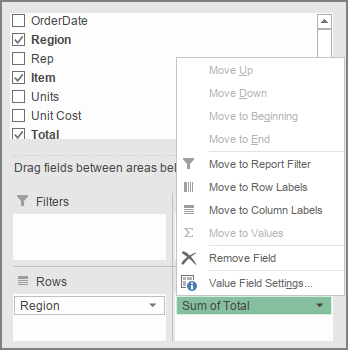
\includegraphics[width=\maxwidth{.75\linewidth}]{gfx/ch07_fig16}
			\caption{Values popup}
			\label{07:fig16}
		\end{figure}

		\item Select \fmtButton{Value Field Settings}.
		\item Select \fmtButton{Average} in the popup, as illustrated in Figure \ref{07:fig17}
		\item Click \fmtButton{OK}.
	\end{enumerate}

	\begin{figure}[H]
		\centering
		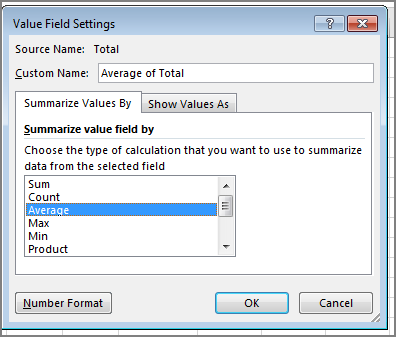
\includegraphics[width=\maxwidth{.75\linewidth}]{gfx/ch07_fig17}
		\caption{Selecting Average Values}
		\label{07:fig17}
	\end{figure}

	\item The PivotTable is instantly changed to display the average sales by region and item.
	\item The average is displayed to seven decimal places. Since this is money, it would be best to round the averages to two decimal places.

	\begin{enumerate}
		\item Click the down arrow in \textit{Average of Total} in the \textit{Values} area. 
		\item Select \fmtButton{Value Field Settings}.
		\item Click the \fmtButton{Number Format} button at the bottom left corner of the \textit{Value Field Settings} popup, as illustrated in Figure \ref{07:fig18}.

	\begin{figure}[H]
		\centering
		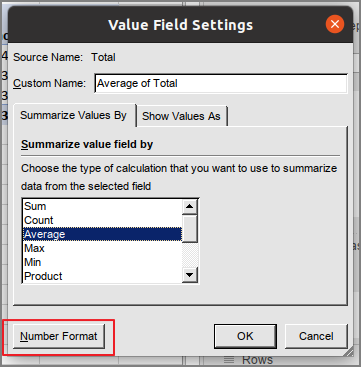
\includegraphics[width=\maxwidth{.75\linewidth}]{gfx/ch07_fig18}
		\caption{The Number Format Button}
		\label{07:fig18}
	\end{figure}

		\item Choose \fmtButton{Number} and set 2 decimal places (the default setting).

	\begin{figure}[H]
		\centering
		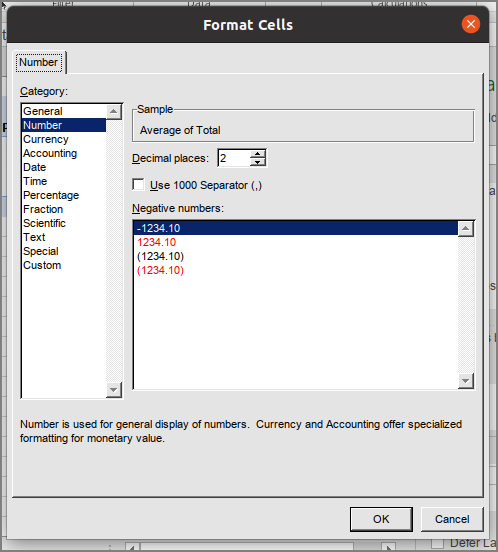
\includegraphics[width=\maxwidth{.95\linewidth}]{gfx/ch07_fig19}
		\caption{Setting Two Decimal Places}
		\label{07:fig19}
	\end{figure}

		\item Click \fmtButton{OK}.
		\item Click \fmtButton{OK}.
	\end{enumerate}

	\item The pivot table is instantly changed to display the averages rounded to two decimal places, so it is more like money.
	
	\item Click \fmtButton{Analyze $ \Rightarrow $ PivotTable $ \Rightarrow $ PivotTable Name} and enter \fmtTyping{Sales}, as illustrated in Figure \ref{07:fig20}.
\end{enumerate}

\begin{figure}[H]
	\centering
	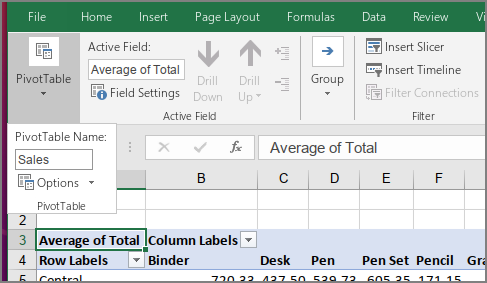
\includegraphics[width=\maxwidth{.50\linewidth}]{gfx/ch07_fig20}
	\caption{Renaming the Pivot Table}
	\label{07:fig20}
\end{figure}

\begin{enumerate}[resume]
	\item Create a new pivot table by clicking in cell \fmtLoc{A1} in the \fmtWorksheet{Sales Data} worksheet.
	\item Click \fmtButton{Insert $ \Rightarrow $ Tables $ \Rightarrow $ PivotTable}.
	\item In the \textit{Create PivotTable} popup, ensure that Excel automatically selected the data table name, \textit{CH7\_Data}, or the data range \$A\$1:\$G\$44, which is all the data on the worksheet. Also, ensure \fmtButton{New Worksheet} is selected as the location of the new pivot table. 
	\item Click \fmtButton{OK}.
	\item A pivot table is created on a new worksheet. Rename that worksheet \fmtWorksheet{Annual Pivot} and move it to the right of \fmtWorksheet{Sales Pivot}.
	\item Click \fmtButton{Analyze $ \Rightarrow $ PivotTable $ \Rightarrow $ PivotTable Name} and enter \fmtTyping{Annual} for the \textit{Pivot Table Name}.
	\item Check \textit{OrderDate} in the \textit{Field List}. By default, Excel places that item in the pivot table \textit{Row Labels} area since it contains dates. Notice that Excel automatically expands the dates into years and quarters.
	\item Drag \textit{Total} from the \textit{Field List} to \textit{Values}. The pivot table now shows the total sales by date. Clicking the plus sign beside the years and quarters in the pivot table drills down to specific quarters and months of interest.
	\item Drag \textit{Region} from the \textit{Field List} to \textit{Columns}. This creates columns for each region in the pivot table so now management can find sales by month and region.
\end{enumerate}	

\begin{figure}[H]
	\centering
	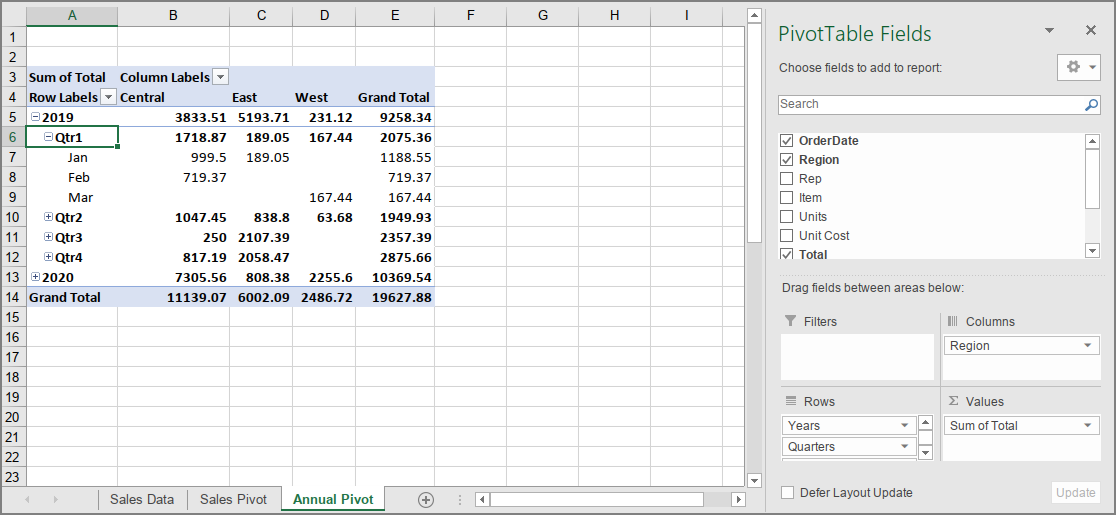
\includegraphics[width=\maxwidth{.95\linewidth}]{gfx/ch07_fig21}
	\caption{Sales Units With Columns}
	\label{07:fig21}
\end{figure}

\begin{enumerate}[resume]
	\item To filter the data, click the down arrow to the right of the \textit{Column Labels} or \textit{Row Labels} headers on the pivot table (see Figure \ref{07:fig22}). Check only those regions or dates that should be included in the pivot table. For example, click the down arrow to the right of the \textit{Column Labels} and uncheck everything except \textit{East} and notice how the pivot table is updated to include only the East region. Also notice that the dropdown includes options to sort the data in the pivot table.
\end{enumerate}

\begin{figure}[H]
	\centering
	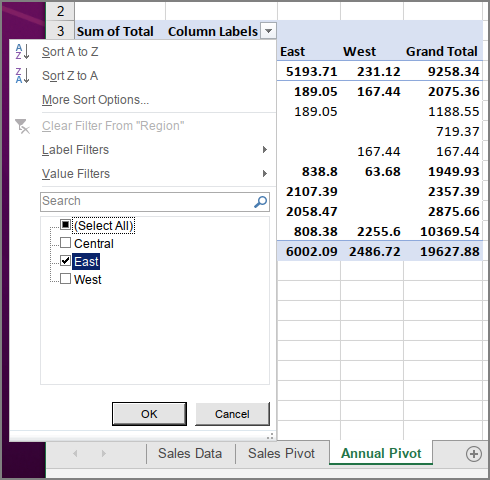
\includegraphics[width=\maxwidth{.95\linewidth}]{gfx/ch07_fig22}
	\caption{Filtering Regions}
	\label{07:fig22}
\end{figure}

\begin{enumerate}[resume]
	\item While managers normally like having dates grouped by month/quarter/year, that can be easily modified. Click cell \fmtLoc{A5} in the pivot table so only that one cell is selected. Click \fmtButton{Analyze $ \Rightarrow $ Group $ \Rightarrow $ Group Field}.
\end{enumerate}

\begin{figure}[H]
	\centering
	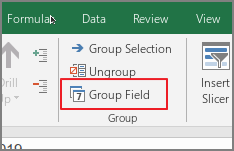
\includegraphics[width=\maxwidth{.50\linewidth}]{gfx/ch07_fig23}
	\caption{The Group Field Button}
	\label{07:fig23}
\end{figure}

\begin{enumerate}[resume]
	\item In the \textit{Grouping} popup box the start/end dates for the data can be specified in order to limit the data shown in the pivot table. For this excercise, leave the dates at their default (two entire years), but click \textit{months} so it is no longer highlighted then click \fmtButton{OK}. Figure \ref{07:fig24} illustrates the \textit{Grouping} popup box after the \fmtButton{Months} item is inactivated. This will remove the \textit{Months} drill down capability and only show years and quarters in the pivot table. By using this option, details can be removed from the pivot table so trends may become more visible.
\end{enumerate}

\begin{figure}[H]
	\centering
	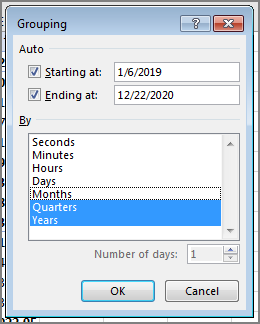
\includegraphics[width=\maxwidth{.60\linewidth}]{gfx/ch07_fig24}
	\caption{Removing Months From The Group}
	\label{07:fig24}
\end{figure}

\begin{enumerate}[resume]
	\item Drag \textit{Rep} from the Field List to the Filters area. Notice that the pivot table now has a selector in cell \fmtLoc{B1} so a specific representative (or group of representatives) can be used to filter data on the pivot table. Click the down arrow for the \textit{Rep} filter, select \fmtButton{Andrews}, and click \fmtButton{OK}. Notice that the pivot table is instantly updated to include only Andrews' sales data.
\end{enumerate}

\begin{figure}[H]
\centering
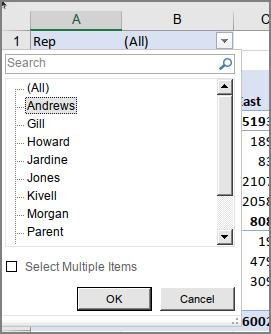
\includegraphics[width=\maxwidth{.50\linewidth}]{gfx/ch07_fig25}
\caption{Filtering For One Representative}
\label{07:fig25}
\end{figure}

\begin{enumerate}[resume]
	\item This pivot table will be used to create a pivot chart in the next section; however, the filter is not needed. Uncheck \textit{Rep} in the Field List to remove that from the filter area.
	\item Save the \fmtWorksheet{CH7-Sales Summary} workbook.
\end{enumerate}

\begin{center}
	\begin{tkwbox}{Key Take-Aways}
		\textbf{Pivot Tables}
		\\
		\begin{itemize}
			\setlength{\itemsep}{0pt}
			\setlength{\parskip}{0pt}
			\setlength{\parsep}{0pt}
			
			\item Pivot tables are a very powerful analysis tool that are easy to create and use.
			
		\end{itemize}
	\end{tkwbox}
\end{center}

\section{Recommended Pivot Tables}

\begin{center}
	\begin{objbox}{Learning Objectives}
		\begin{itemize}
			\setlength{\itemsep}{0pt}
			\setlength{\parskip}{0pt}
			\setlength{\parsep}{0pt}
			
			\item Evaluate and select a recommended pivot table.
			
		\end{itemize}
	\end{objbox}
\end{center}

\begin{enumerate}
	\item Open the \fmtWorksheet{Sales Summary} workbook that was created in section \ref{07:ImportFromDataFile} if it is not already opened.
	\item Click cell \fmtLoc{A1} in the \fmtWorksheet{Sales Data} worksheet.
	\item Click \fmtButton{Insert $ \Rightarrow $ Tables $ \Rightarrow $ Recommended PivotTables}.
	\item Excel will analyze the data and create several recommended pivot tables. These can be clicked and previewed in the \textit{Recommended PivotTables} popup. Figure \ref{07:fig26} illustrates the \textit{Recommended PivotTables} popup.
\end{enumerate}

\begin{figure}[H]
	\centering
	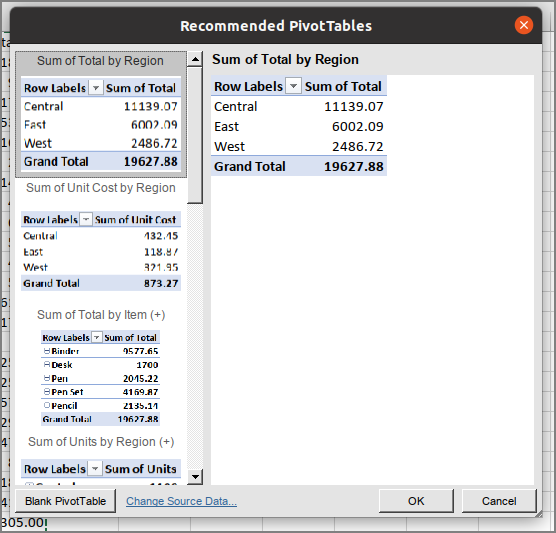
\includegraphics[width=\maxwidth{.95\linewidth}]{gfx/ch07_fig26}
	\caption{Recommended PivotTables}
	\label{07:fig26}
\end{figure}

\begin{enumerate}[resume]
	\item Click on the first recommended pivot table, \fmtButton{Sum of Total by Region}, and click \fmtButton{OK}.
	\item Excel creates the pivot table in a new worksheet. Name that worksheet \fmtWorksheet{Sales By Region}.
	Move \fmtWorksheet{Sales By Region} to the right of \fmtWorksheet{Annual Pivot}.
	\item Click \fmtButton{Analyze $ \Rightarrow $ PivotTable $ \Rightarrow $ PivotTable Name} and enter \fmtTyping{By Region}.
	\item The new pivot table includes all of the same features as those created manually so formatting and variable manipulation is available to modify this table.
	\item Save the \fmtWorksheet{CH7-Sales Summary} workbook.
\end{enumerate}

\begin{center}
	\begin{tkwbox}{Key Take-Aways}
		\textbf{Recommended Pivot Tables}
		\\
		\begin{itemize}
			\setlength{\itemsep}{0pt}
			\setlength{\parskip}{0pt}
			\setlength{\parsep}{0pt}
			
			\item Excel automatically analyzes data in a worksheet and recommends appropriate pivot tables for the data.
			\item If a recommended pivot table is selected, it can be easily manipulated to meet the goals of the research project.
			
		\end{itemize}
	\end{tkwbox}
\end{center}

\section{Pivot Charts}

\begin{center}
	\begin{objbox}{Learning Objectives}
		\begin{itemize}
			\setlength{\itemsep}{0pt}
			\setlength{\parskip}{0pt}
			\setlength{\parsep}{0pt}
			
			\item Create and format a pivot chart.
			
		\end{itemize}
	\end{objbox}
\end{center}

One of the strengths of creating a pivot table is that the table can be used to create a chart and as the table is modified the chart is also automatically modified. Follow these directions to explore the power of pivot charts.

\begin{enumerate}
	\item Open the \fmtWorksheet{Sales Summary} workbook that was created in section \ref{07:ImportFromDataFile} if it is not already opened.
	\item Open the \fmtWorksheet{Sales Data} worksheet.
	\item Activate cell \fmtLoc{A1} by clicking in it.  
	\item Click \fmtButton{Insert $ \Rightarrow $ Charts $ \Rightarrow $ Pivot Chart}.
\end{enumerate}

\begin{figure}[H]
	\centering
	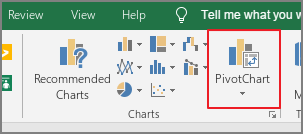
\includegraphics[width=\maxwidth{.95\linewidth}]{gfx/ch07_fig27}
	\caption{The Pivot Chart Button}
	\label{07:fig27}
\end{figure}

\begin{enumerate}[resume]	
	\item In the \textit{Create PivotChart} popup, ensure that Excel automatically selected either the data table by name, \textit{CH7\_Data}, or the data range, \$A\$1:\$G\$44, which is all the data on the worksheet. Also, ensure \fmtButton{New Worksheet} is selected as the location of the new pivot chart.
	\item Click \fmtButton{OK}.
	\item Excel will open a new pivot chart worksheet. This worksheet is similar to a pivot table worksheet and creating a chart is like creating a table.
	\item Rename the pivot chart worksheet to \fmtWorksheet{Sales By Item}. 
	\item Move \fmtWorksheet{Sales By Item} to the right of \fmtWorksheet{Sales By Region}.
	\item In the \textit{Field List}, click the checkboxes for \fmtButton{Rep} and \fmtButton{Total}. Excel creates a bar chart that shows the total sales for each Representative, as illustrated in Figure \ref{07:fig28}.
\end{enumerate}	

\begin{figure}[H]
	\centering
	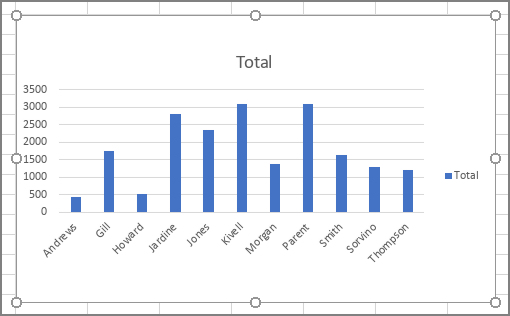
\includegraphics[width=\maxwidth{.95\linewidth}]{gfx/ch07_fig28}
	\caption{Sales By Representative}
	\label{07:fig28}
\end{figure}

\begin{enumerate}
	\item Uncheck \fmtButton{Rep} and check \fmtButton{Item}.
	\item The bar chart automatically updates to display the total sales for each item in the inventory. This chart, though, would be better if it were a pie chart.
	
	\begin{enumerate}
		\item Click the down arrow for the \fmtButton{Sum of Total} item in the \textit{Values} area of the pivot table.
		\item Select \fmtButton{Value Field Settings} in the popup options menu.
		\item Click the \fmtButton{Show Values As} tab in the \textit{Value Field Settings} popup box.
		\item Choose \fmtButton{\% of Grand Total} in the drop-down menu near the middle of the \textit{Value Field Settings} box.
\end{enumerate}

\begin{figure}[H]
	\centering
	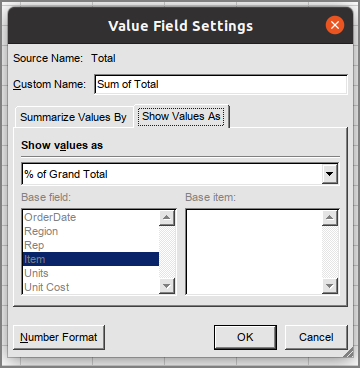
\includegraphics[width=\maxwidth{.75\linewidth}]{gfx/ch07_fig29}
	\caption{Values As a Percentage Of The Total}
	\label{07:fig29}
\end{figure}

\begin{enumerate}[resume]		
		\item Click \fmtButton{OK}.
		\item The values in the pivot table change to percentages rather than numbers.
	\end{enumerate}
	
	\item Click \fmtButton{Design $ \Rightarrow $ Type $ \Rightarrow $ Change Chart Type}.
	\item Select \fmtButton{Pie Chart} and click \fmtButton{OK}.
\end{enumerate}

\begin{figure}[H]
	\centering
	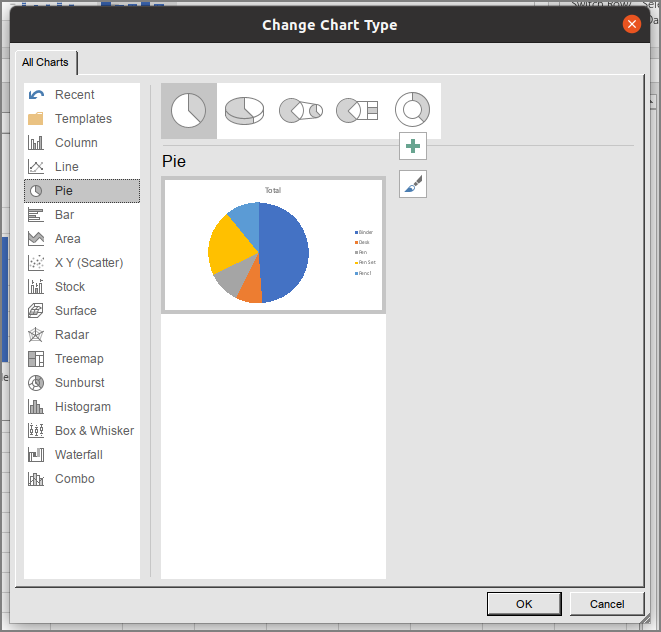
\includegraphics[width=\maxwidth{.95\linewidth}]{gfx/ch07_fig30}
	\caption{Selecting a Pie Chart}
	\label{07:fig30}
\end{figure}

\begin{enumerate}[resume]	
	\item Click the $ + $ sign at the top right of the pie chart and then click \fmtButton{Data Labels} to display the percent of each slice.
\end{enumerate}

\begin{figure}[H]
	\centering
	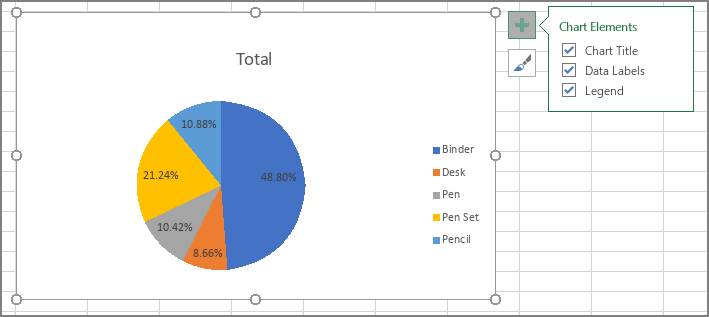
\includegraphics[width=\maxwidth{.95\linewidth}]{gfx/ch07_fig31}
	\caption{Adding Data Labels}
	\label{07:fig31}
\end{figure}

\begin{enumerate}[resume]	
	\item Click off of the chart so it is no longer selected and then right-click on the chart title. Select \fmtButton{Edit Text} from the popup menu.
\end{enumerate}

\begin{figure}[H]
	\centering
	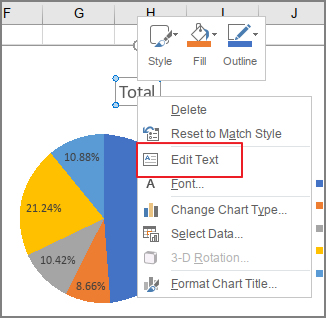
\includegraphics[width=\maxwidth{.75\linewidth}]{gfx/ch07_fig32}
	\caption{Editing The Title}
	\label{07:fig32}
\end{figure}

\begin{enumerate}[resume]	
	\item Enter \fmtTyping{Sales by Item} as the chart title and then click off of the chart so it is no longer selected.
	\item The chart colors and other chart elements can be changed using options found at \fmtButton{Design $ \Rightarrow $ Group $ \Rightarrow $ Button}.
	\item Save the \fmtWorksheet{CH7-Sales Summary} workbook.
	\item Close the \fmtWorksheet{CH7-Sales Summary} workbook.
\end{enumerate}

\begin{center}
	\begin{tkwbox}{Key Take-Aways}
		\textbf{Pivot Charts}
		\\
		\begin{itemize}
			\setlength{\itemsep}{0pt}
			\setlength{\parskip}{0pt}
			\setlength{\parsep}{0pt}
			
			\item Creating a pivot chart uses the same process as a pivot table.
			\item Once a pivot chart has been created, it can be modified using all of the chart tools.
			
		\end{itemize}
	\end{tkwbox}
\end{center}

\section{Preparing to Print}

\begin{center}
	\begin{objbox}{Learning Objectives}
		\begin{itemize}
			\setlength{\itemsep}{0pt}
			\setlength{\parskip}{0pt}
			\setlength{\parsep}{0pt}
			
			\item Review each worksheet in a workbook in Print Preview.
			\item Modify worksheets as needed to professionally print data and charts.
			
		\end{itemize}
	\end{objbox}
\end{center}

Just like consistency in formatting is important when working with workbooks containing multiple worksheets with pivot tables and charts,  so is consistency in page setup. The \textit{CH7-Sales Summary} workbook should be prepared for printing by modifying some of the settings and adding a header and footer. 

\begin{enumerate}
	\item Open the \fmtWorksheet{CH7-Sales Summary} workbook that was created in section \ref{07:ImportFromDataFile}.
	\item Click \fmtButton{File $ \Rightarrow $ Print} to enter the print preview. To view all of the worksheets at one time, select \fmtButton{Print Entire Workbook} in the first box in the Settings section. There are $ 6 $ pages to scroll through in \textit{Print Preview}. 

	\begin{itemize}
		\item All of the pages look good except pages one and five.
		\item Page one is just the raw data. There is no point in printing that worksheet so it should be hidden.
		\item Page five has part of a pivot chart, but it continues onto another page.
		\item A header and footer should be added.
	\end{itemize}

	\item Exit \textit{Print Preview} by clicking the arrow in the top left corner of the page.
	\item Right-click on the \fmtWorksheet{Sales Data} worksheet tab and select \fmtButton{Hide}. This hides the worksheet so it is not printed, but the worksheet and data are all still available in the workbook so the pivot tables will still be functional.
	\item Activate the \fmtWorksheet{Sales By Item} worksheet by clicking that tab. Notice that part of the chart is printing on a second page as indicated by a dotted line running down the edge of column J. 
	\item Resize the chart using the values in Table \ref{07:tab01}. For each side of the chart, press the \fmtKeystroke{Alt} key while dragging the resize handle on the chart.
\end{enumerate}	

\begin{table}[H]
\rowcolors{1}{}{tablerow} % zebra striping background
{\small
	%\fontsize{8}{10} \selectfont %Replace small for special font size
	\begin{longtable}{R{0.75in}L{1.50in}} %Left-aligned, Max width: 4.25in
		\textbf{Chart Side} & \textbf{Locked To} \endhead
		\hline
		Top & Top of \fmtLoc{Row 9}\\
		Left & Left of \fmtLoc{Column B}\\
		Bottom & Bottom of \fmtLoc{Row 23}\\
		Right & Right of \fmtLoc{Column G}\\
		\rowcolor{captionwhite}
		\caption{Resizing Sales by Item Chart}
		\label{07:tab01}
	\end{longtable}
} % End small
\end{table}

\begin{enumerate}[resume]
	\item Activate the \fmtWorksheet{Sales Pivot} worksheet by clicking that tab. 
	\item Click \fmtButton{Insert $ \Rightarrow $ Text $ \Rightarrow $ Header \& Footer}.
	\item Click in the right section of the header to activate it. 
	\item Click \fmtButton{Header \& Footer Elements $ \Rightarrow $ Current Date}.
	\item Click \fmtButton{Navigation $ \Rightarrow $ Go to Footer}. 
	\item Click in the center section of the footer to activate it. 
	\item Click \fmtButton{Header \& Footer Elements $ \Rightarrow $ Sheet Name}
	\item Click anywhere on the worksheet outside the footer.
	\item Click \fmtButton{View \& Workbook Views $ \Rightarrow $ Normal}.
	\item Repeat the same procedure to place a header and footer on the other three worksheets.
	\item Click \fmtButton{File $ \Rightarrow $ Print} to enter the print preview. To view all of the worksheets at one time, select \fmtButton{Print Entire Workbook} in the first box in the Settings section. There are $ 4 $ pages to scroll through in \textit{Print Preview}. Confirm that each worksheet is printing on one page with the date in the header and the worksheet name in the footer.
	\item Save and close the \fmtWorksheet{CH7-Sales Summary} workbook.
\end{enumerate}

\begin{center}
	\begin{tkwbox}{Key Take-Aways}
		\textbf{Preparing to Print}
		\\
		\begin{itemize}
			\setlength{\itemsep}{0pt}
			\setlength{\parskip}{0pt}
			\setlength{\parsep}{0pt}
			
			\item Formatting for print is an essential part of creating a workbook.
			
		\end{itemize}
	\end{tkwbox}
\end{center}

\section{Chapter Practice}

\subsection{Project Team Analysis}

\begin{enumerate}
	\item Load the data.

	\begin{enumerate}
		\item Start Excel and open a new blank workbook.
		\item Save the workbook as \fmtWorksheet{PR7-Project}.
		\item \fmtOldExcel{Excel 2016} Click \fmtButton{Data $ \Rightarrow $ Get \& Transform $ \Rightarrow $ New Query $ \Rightarrow $ From File $ \Rightarrow $ From CSV}
		\item \fmtNewExcel{Excel 365} Click \fmtButton{Data $ \Rightarrow $ Get \& Transform Data $ \Rightarrow $ Get Data $ \Rightarrow $ From File $ \Rightarrow $ From Text/CSV}
		\item Navigate to \fmtWorksheet{PR7-Data.csv}.
		\item Click the file name and then \fmtButton{Import}.
		\item When the import wizard opens, click \fmtButton{Load}.
		\item Rename \fmtWorksheet{Sheet2} to \fmtWorksheet{Project Data}.
		\item Delete \fmtWorksheet{Sheet1}.
		\item Close the \textit{Workbook Queries} panel.
	\end{enumerate}

	\item{\textbf{Question 1}: What type of project is the most fiscally productive?}

	\begin{enumerate}
		\item Activate cell \fmtLoc{A1} by clicking in the cell.
		\item Click \fmtButton{Insert $ \Rightarrow $ Tables $ \Rightarrow $ Recommended PivotTables}.	
		\item Select the pivot table named \fmtButton{Sum of Amount Billed by Project Type} and click \fmtButton{OK}.
		\item Rename the pivot table to \fmtTyping{Billed} and then rename the worksheet to \fmtTyping{Billed}.
		\item Move the \fmtWorksheet{Billed} worksheet to the right of the \fmtWorksheet{Project Data} worksheet.
		\item Click the down arrow to the right of \textit{Sum of Amount Billed} in the \textit{Values} area and select \fmtButton{Value Field Settings}.
		\item Change the \textit{Custom Name} of this field to \fmtTyping{Total Billed}.
		\item Click \fmtButton{OK}.
		\item Right-click in cell \fmtLoc{B2} to activate it.
		\item In the popup menu, select \fmtButton{Sort $ \Rightarrow $ Sort Largest to Smallest}. This sorts the total billed from the largest to smallest amount.
		\item Save the \fmtWorksheet{PR7-Project} workbook.
	\end{enumerate}

	\item{\textbf{Question 2}: Which client spends the most?	}

	\begin{enumerate}
		\item Click in cell \fmtLoc{A1} in the \fmtWorksheet{Project Data} worksheet to activate it.
		\item Click \fmtButton{Insert $ \Rightarrow $ Tables $ \Rightarrow $ PivotTable}.
		\item Create a pivot table on a new worksheet.
		\item Name the pivot table and worksheet \fmtTyping{Clients}.
		\item Move the \fmtWorksheet{Clients} worksheet to the right of the \fmtWorksheet{Billed} worksheet.
		\item Drag \textit{Client} from the \textit{Field List} to the \textit{Rows} area.
		\item Drag \textit{Amount Billed} from the \textit{Field List} to the \textit{Values} area.
		\item Change the name of the values header from \textit{Sum of Amount Billed} to \fmtTyping{Total Billed}.
		\item Sort the \textit{Total Billed} column so the largest number is at the top.
		\item Save the \fmtWorksheet{PR7-Project} workbook.
	\end{enumerate}

	\item{\textbf{Question 3}: Which quarter was the most profitable?}

	\begin{enumerate}
		\item Click in cell \fmtLoc{A1} in the \fmtWorksheet{Project Data} worksheet to activate it.
		\item Click \fmtButton{Insert $ \Rightarrow $ Tables $ \Rightarrow $ PivotTable}.
		\item Create a pivot table on a new worksheet.
		\item Name the pivot table and worksheet \fmtTyping{Quarterly}.
		\item Move the \fmtWorksheet{Quarterly} worksheet to the right of the \fmtWorksheet{Clients} worksheet.
		\item Drag \textit{Date Completed} from the \textit{Field List} to the \textit{Rows} area.
		\item Drag \textit{Amount Billed} from the \textit{Field List} to the \textit{Values} area.
		\item Change the name of the values header from \textit{Sum of Amount Billed} to \fmtTyping{Total Billed}.
		\item Click the \textit{plus} buttons beside $ 2016 $ and $ 2017 $ to view the amount billed by quarter.
		\item Save the \fmtWorksheet{PR7-Project} workbook.
	\end{enumerate}
	
	\item{\textbf{Question 4}: Which team completed the largest proportion of the projects?}

	\begin{enumerate}
		\item Click in cell \fmtLoc{A1} in the \fmtWorksheet{Project Data} worksheet to activate it.
		\item Click \fmtButton{Insert $ \Rightarrow $ Charts $ \Rightarrow $ PivotChart}.
		\item Create a pivot chart on a new worksheet.
		\item Name the pivot chart and worksheet \fmtTyping{Teams}.
		\item Move the \fmtWorksheet{Teams} worksheet to the right of the \fmtWorksheet{Quarterly} worksheet.
		\item Drag \textit{Team Leader} from the \textit{Field List} to the \textit{Axis (Categories)} area.
		\item Drag \textit{Hours Spent} from the \textit{Field List} to the \textit{Values} area.
		\item Change the name of the values header from \textit{Sum of Hours Spent} to \fmtTyping{Total Hours}.
		\item Sort the \textit{Total Hours} column so the largest number is at the top.
		\item Change the title of the chart to \fmtTyping{Total Hours Spent}.
		\item Since there is only one data point, the legend is not needed, so remove it. Click the $ + $ sign near the top right corner of the chart and uncheck the \fmtButton{Legend} item.
		\item Save and close the \fmtWorksheet{PR7-Project} workbook.
	\end{enumerate}

	\item Submit the \fmtWorksheet{PR7-Project} workbook to the instructor.

\end{enumerate}

\section{Scored Assessment}

\subsection{Employee Analysis}

\begin{enumerate}
	\item Load the data.
	
	\begin{enumerate}
		\item Start Excel and open a new blank workbook.
		\item Save the workbook as \fmtWorksheet{SC7-Employees}.
		\item \fmtOldExcel{Excel 2016} Click \fmtButton{Data $ \Rightarrow $ Get \& Transform $ \Rightarrow $ New Query $ \Rightarrow $ From File $ \Rightarrow $ From CSV}
		\item \fmtNewExcel{Excel 365} Click \fmtButton{Data $ \Rightarrow $ Get \& Transform Data $ \Rightarrow $ Get Data $ \Rightarrow $ From File $ \Rightarrow $ From Text/CSV}
		\item Navigate to \fmtWorksheet{SC7-Data.csv}.
		\item Click the file name and then \fmtButton{Import}.
		\item When the import wizard opens, click \fmtButton{Load}.
		\item Rename \fmtWorksheet{Sheet2} to \fmtWorksheet{Employee Data}.
		\item Delete the \fmtWorksheet{Sheet1} worksheet.
		\item Close the \textit{Workbook Queries} panel.
	\end{enumerate}
	
	\item{\textbf{Question 1}: What is the average salary for each role?}
	
	\begin{enumerate}
		\item Create a pivot table that lists the roles in the business (Accounting, Associate, etc.), the number of people in each role, and the average salary for that role. Hint: the \textit{Role} field should be dragged to both the \textit{Rows} area and the \textit{Values} area.
		\item The pivot table and worksheet should be named \fmtWorksheet{Avr Salary} and that worksheet should be to the right of the \fmtWorksheet{Employee Data} worksheet.
		\item The \textit{Salary} field should be changed from sum to average and renamed \textit{Avr Salary}. It should also be formatted as currency with two decimal places.
		\item \textit{Count of role} in the \textit{values} field should be renamed \textit{Count}.
		\item Sort the list so the highest salary is first. 
		\item Save the \fmtWorksheet{SC7-Employees} workbook.
		\item Figure \ref{07:fig58} illustrates how the pivot table should look.
	\end{enumerate}

\end{enumerate}

\begin{figure}[H]
	\centering
	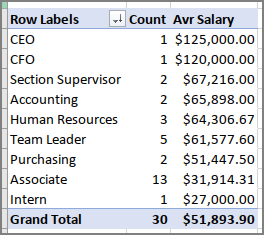
\includegraphics[width=\maxwidth{.75\linewidth}]{gfx/ch07_fig58}
	\caption{Average Salary By Role}
	\label{07:fig58}
\end{figure}

\begin{enumerate}[resume]
	\item{\textbf{Question 2}: What is the average age of the employees when broken down by sex and marital status?}
	
	\begin{enumerate}
		\item Create a pivot table that lists the average age by marital status and sex for all employees.
		\item The pivot table and worksheet should be named \fmtWorksheet{Avr Age} and that worksheet should be to the right of the \fmtWorksheet{Avr Salary} worksheet.
		\item The average age should be formatted as a number with zero decimal places. 
		\item Save the \fmtWorksheet{SC7-Employees} workbook.
		\item Figure \ref{07:fig59} illustrates how the pivot table should look.
	\end{enumerate}
	
\end{enumerate}

\begin{figure}[H]
	\centering
	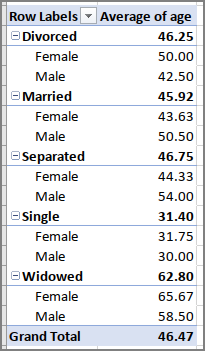
\includegraphics[width=\maxwidth{.75\linewidth}]{gfx/ch07_fig59}
	\caption{Avr Age}
	\label{07:fig59}
\end{figure}

\begin{enumerate}[resume]
	\item{\textbf{Question 3}: How many employees have been hired each year from 2007?}
	
	\begin{enumerate}
		\item Create a pivot table that lists the employee count by year. (\textit{Hint}: count the username field since each employee has a unique username.)
		\item The pivot table and worksheet should be named \fmtWorksheet{Year Hired} and that worksheet should be to the right of the \fmtWorksheet{Avr Age} worksheet.
		\item The username field should be labeled \textit{count}. 
		\item The \textit{hired} field should display only years, not quarters or months.
		\item The list should be sorted by year (which is the default).
		\item Save the \fmtWorksheet{SC7-Employees} workbook.
		\item Figure \ref{07:fig60} illustrates how the pivot table should look.
	\end{enumerate}
	
\end{enumerate}

\begin{figure}[H]
	\centering
	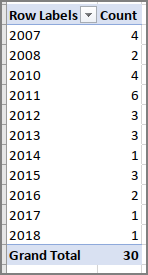
\includegraphics[width=\maxwidth{.75\linewidth}]{gfx/ch07_fig60}
	\caption{Number Hired By Year}
	\label{07:fig60}
\end{figure}

\begin{enumerate}[resume]
	\item{\textbf{Question 4}: How many employees work in each role?}
	
	\begin{enumerate}
		\item Create a pivot chart (\textit{note}, this is a chart, not a table) that shows the count by role. (\textit{Hint}: count the username field since each employee has a unique username.)
		\item The pivot chart and worksheet should be named \fmtWorksheet{Count By Role} and that worksheet should be to the right of the \fmtWorksheet{Year Hired} worksheet.
		\item The username field should be labeled \textit{Number}.
		\item The data should be sorted such that the role with the most employees (``Associate'') should be first.
		\item The chart's title should be \textit{Count by Role}
		\item The chart should not have a legend.
		\item Save the \fmtWorksheet{SC7-Employees} workbook.
		\item Figure \ref{07:fig61} illustrates how the pivot chart should look.
	\end{enumerate}
	
\end{enumerate}

\begin{figure}[H]
	\centering
	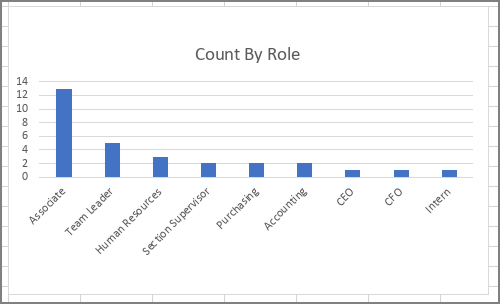
\includegraphics[width=\maxwidth{.95\linewidth}]{gfx/ch07_fig61}
	\caption{Count By Role}
	\label{07:fig61}
\end{figure}

\begin{enumerate}[resume]
	\item Prior to submitting this workbook, use the Print Preview to make sure the worksheets are printing properly.
	
	\begin{enumerate}
		\item Hide the \fmtWorksheet{Employee Data} worksheet.
		\item On the \fmtWorksheet{Count by Role} worksheet, the pivot chart needs to be moved under the pivot table.
		\item Add a footer to each sheet that displays the sheet name in the center section of the footer.
	\end{enumerate}
	
	\item Save and close the \fmtWorksheet{SC7-Employees} workbook.
	\item Submit the \fmtWorksheet{SC7-Employees} workbook to the instructor.
\end{enumerate}